%! TEX root = main.tex

\newcommand{\lang}{danish}
\newcommand{\titl}{Test Document 1}
\newcommand{\auth}{Daniel Brasholt s214676}
\newcommand{\courseno}{01010}
\newcommand{\course}{Testkursus}
\newcommand{\dato}{Maj 2023}
\newcommand{\secheader}{Opgave}
\newcommand{\subsecheader}{Opg.}
\newcommand{\sourcefile}{}
\documentclass[a4paper, \lang]{article}

% Set page size and margins
% Replace `letterpaper' with`a4paper' for UK/EU standard size
\usepackage[
	a4paper,
	top=2cm,
	bottom=2cm,
	left=2cm,
	right=2cm,
	marginparwidth=2cm,
	% headheight=10mm,
	footskip=10mm]{geometry}


% Authors & course variables
\newcommand{\lb}{\\}
\title{\courseno \titl}
\author{\auth}

% Necessary packages
\usepackage[T1]{fontenc}
\usepackage{atkinson}
% \usepackage{newtxtext,newtxmath}
\let\Bbbk\relax
\usepackage[utf8]{inputenc}
\usepackage{babel}
\usepackage{amsmath}
\usepackage{amssymb}
\usepackage{mathtools}
\usepackage{graphicx}
\usepackage{float}
\usepackage{fancyhdr}
\usepackage{subcaption}
\usepackage{lastpage}
\usepackage{listings}
\usepackage[export]{adjustbox}
\usepackage[bottom]{footmisc}
\usepackage{todonotes}
\usepackage{silence}
\usepackage{appendix}
\usepackage{tocloft}
\usepackage{titlesec}
\usepackage{lipsum}
\usepackage{pdfpages}
\usepackage{csquotes}
\usepackage[pdfencoding=auto, psdextra]{hyperref}
\usepackage{cleveref}
\usepackage{outlines}
\hypersetup{
    colorlinks   = true, %Colours links instead of ugly boxes
    urlcolor     = blue, %Colour for external hyperlinks
    linkcolor    = blue, %Colour of internal links
    citecolor   = red %Colour of citations
}
\usepackage[format=plain,
    labelfont={bf,it,footnotesize},
    textfont={it,footnotesize}]{caption}
\captionsetup{font={stretch=0.9}}
\captionsetup{font={stretch=0.9}}
\usepackage[
	backend=biber,
	style=numeric,
 	sorting=nty]
 	{biblatex}
\addbibresource{\sourcefile}

% Equation formatting
\renewcommand{\theequation}{\arabic{section}.\arabic{equation}}
\numberwithin{equation}{section}
\DeclarePairedDelimiter{\paren}{(}{)}
\DeclarePairedDelimiter\ceil{\lceil}{\rceil}

% Figures and sections
%\renewcommand{\figurename}{Figur} % Figure format
\renewcommand{\thesection}{\arabic{section}} % Section format
\renewcommand{\thesubsection}{\arabic{section}.\arabic{subsection}}
\renewcommand{\thesubsubsection}{\arabic{section}.\arabic{subsection}.\alph{subsubsection}}
\Crefname{section}{\secheader}{\secheader}

\titleformat{\section}[block]
{\normalfont\Large\scshape\filright}{\fbox{\secheader\ \thesection}}{1em}{}

\titleformat{\subsection}
{\titlerule
    \vspace{.8ex}%
    \normalfont}
{\subsecheader\ \thesubsection:}{1em}{}

\titleformat{\subsubsection}
{}{\thesubsubsection)}{1em}{}

% Page style with footer
\pagestyle{fancy}
\lhead{\titl \lb \courseno\ \course}
\chead{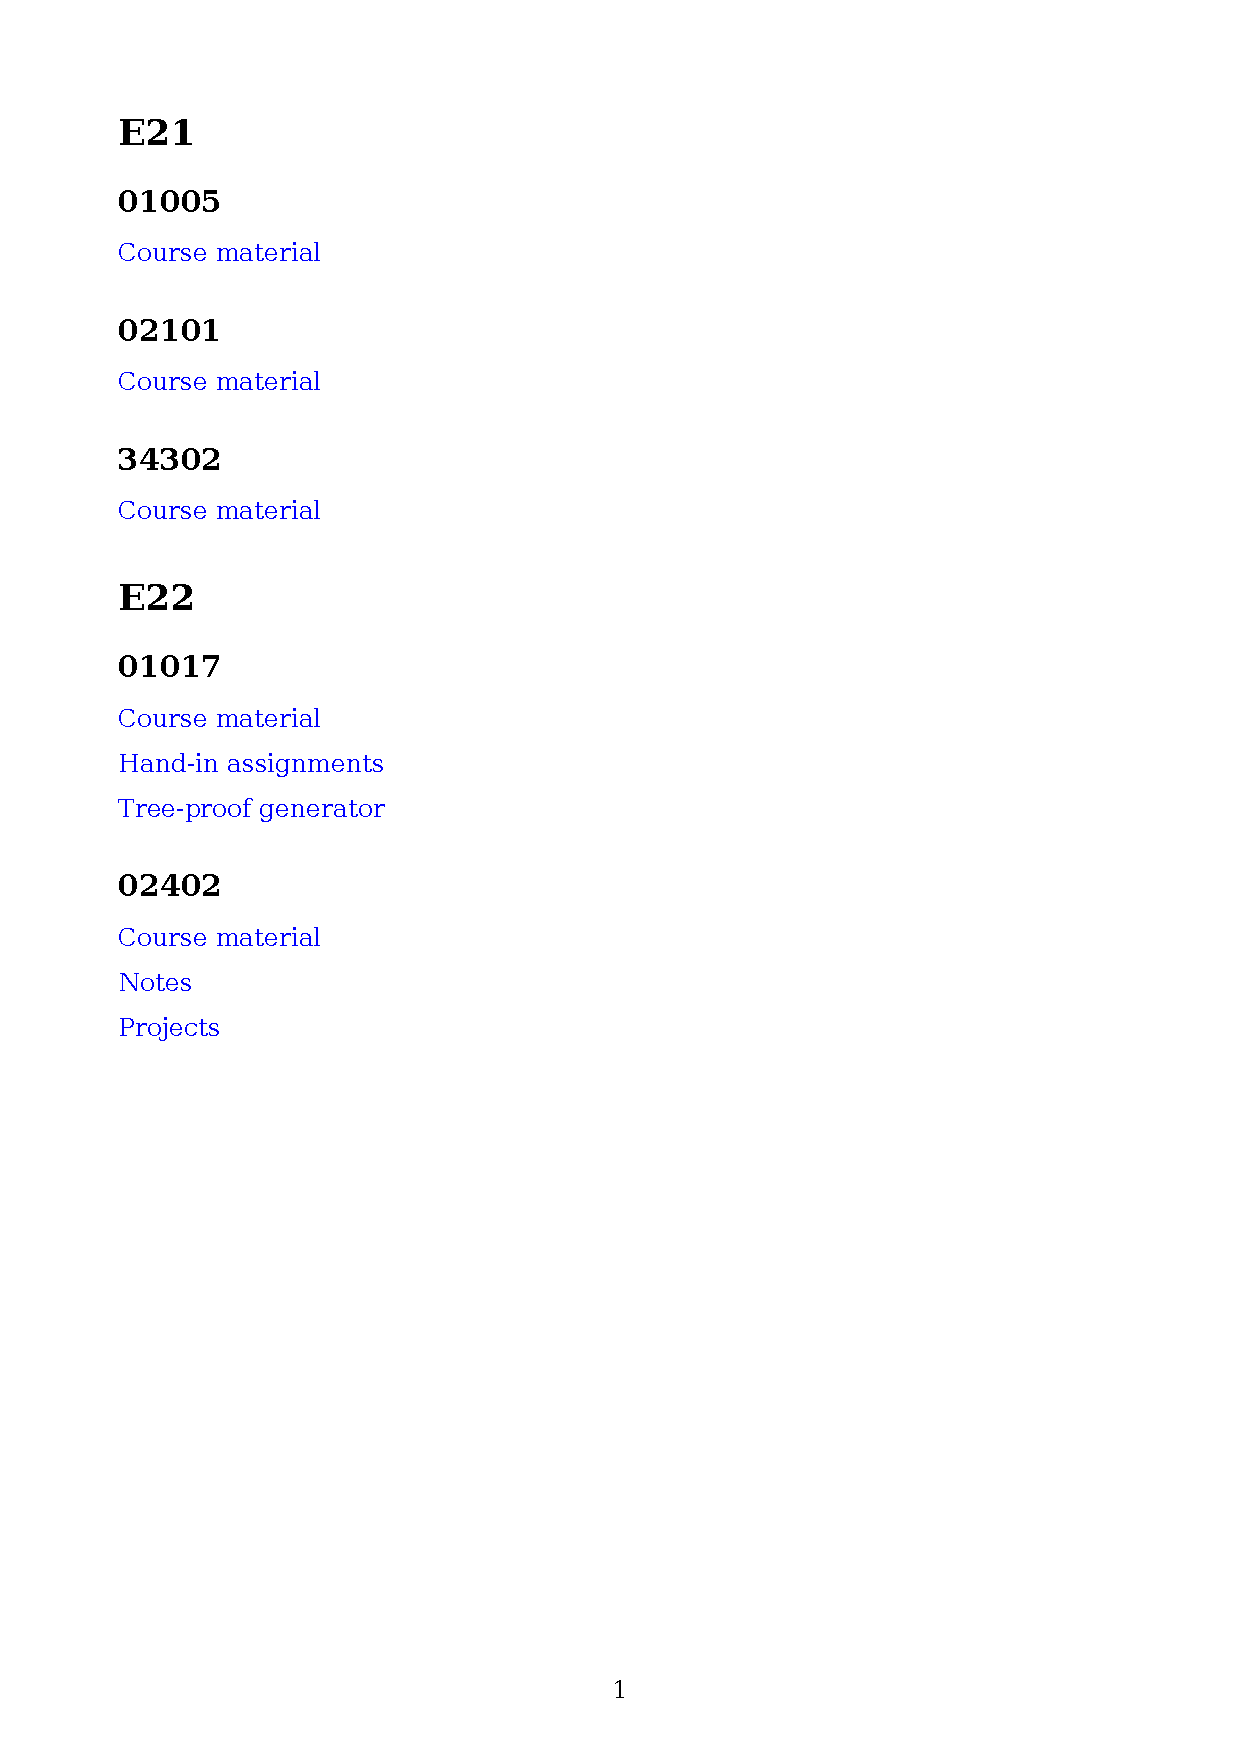
\includegraphics[width=.05\textwidth]{img/DTU}}
\rhead{\auth}
\cfoot{Side \thepage\, af \pageref*{LastPage}}
\renewcommand{\headrulewidth}{0.4pt}
\renewcommand{\footrulewidth}{0.4pt}
\setlength{\headheight}{36.75034pt}

\begin{document}

% Front page & ToC
\title{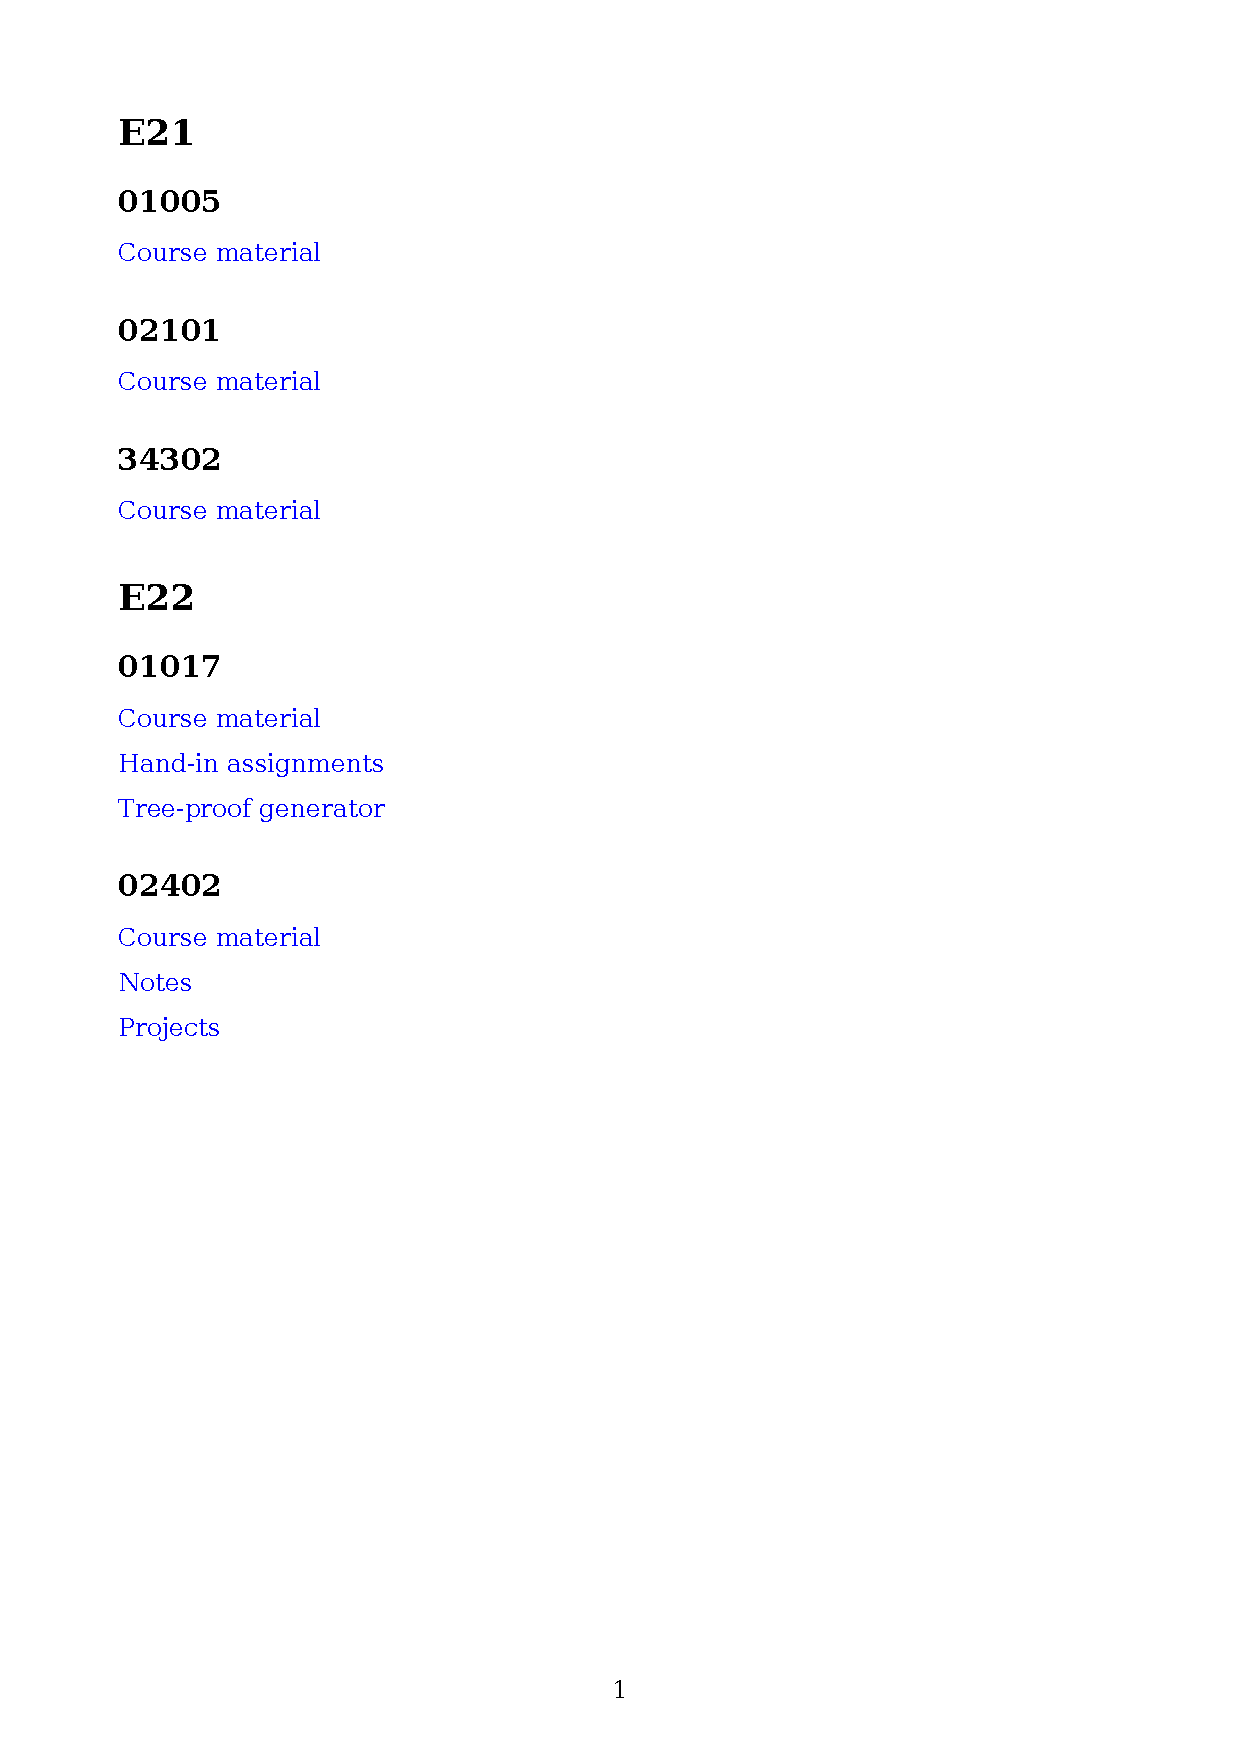
\includegraphics[width=.15\textwidth]{img/DTU}\lb\vspace{.5em}\Huge\scshape
\titl\lb\vspace{-4mm}\rule{4cm}{0.5mm}\lb\Large{\courseno \ \course}}
\author{\auth}
\date{\dato}
\maketitle

\pagenumbering{arabic}
\setcounter{tocdepth}{2}
\tocloftpagestyle{fancy}
\setlength{\cftsubsecnumwidth}{42pt}
\addtolength{\cftsecnumwidth}{47pt}
\addtolength{\cftsubsecnumwidth}{28pt}
\tableofcontents
\addtocontents{toc}{~\hfill\textbf{Side}\par}
\thispagestyle{empty}
\newpage
\setcounter{page}{1}



\section{Section 1}
\label{sec:1}

\begin{figure}[H]
	\centering
	\includegraphics[width=0.2\textwidth]{./img/DTU.eps}
	\caption{Et test-billede?}
	\label{fig:dtu}
\end{figure}

\Cref{fig:dtu}. Og måske også \cref{fig:dtu}. Henvisning til \cref{eq:1}. Til
sidst kan man også sige \cref{sec:1,sec:s1,sec:subsub}.

\subsection{Sub}
\label{sec:s1}

\subsubsection{Subsub}
\label{sec:subsub}

\Cref{sec:subsub} er en god henvisning til \cref{sec:subsub}. Man kunne også
henvise til \cref{sec:1}, hvis man vil. 

\section{Section 2}

\subsection{Sub 2}

\begin{align}
\label{eq:1}
	(\frac{e^{0}}{e^{2}}) = \int_{\infty}^{\infty}{5xdx} \\
	\paren*{\frac{1}{5} \cdot \frac{3}{2} \cdot \frac{5}{2}}
\end{align}

This is true

\lipsum[1-15]

\end{document}
